\ifdefined\ishandout
\documentclass[handout]{beamer}
\else
\documentclass{beamer}
\fi

\usepackage[frenchb]{babel}
\usepackage[T1]{fontenc}
\usepackage[latin1]{inputenc}
\usepackage{hyperref}
\usepackage{multirow}
\usepackage{listings}
\usepackage{fancyvrb}
\usepackage{tikz}
\usepackage{framed}
\usepackage{algorithm}
\usepackage{algorithmic}
\usepackage{xcolor}
\usepackage{color, colortbl}
\ifdefined\ishandout
\usepackage{handoutWithNotes}
\fi
\usepackage{slashbox}
\usepackage{amsmath}
\usepackage{bm}
\usepackage{hhline}

\usetikzlibrary{shapes.geometric}
\usetikzlibrary{positioning}
\usetikzlibrary{shapes.arrows, chains}
\usetikzlibrary{arrows,calc}
\usetikzlibrary{shapes.multipart}
\usepackage{array}
\usetheme{Boadilla}

\usefonttheme[onlymath]{serif}

\newcommand{\R}{\mathbb{R}}
\newcommand{\C}{\mathbb{C}}
\newcommand{\N}{\mathbb{N}}
\newcommand{\Z}{\mathbb{Z}}
\newcommand{\E}{\mathbb{E}}
\newcommand{\Var}{\text{Var}}
\newcommand{\Cov}{\text{Cov}}
\ifdefined\ishandout
\pgfpagesuselayout{3 on 1 with notes}[a4paper,border shrink=5mm]
\usecolortheme{dove}
\else
%\usecolortheme{dolphin}
\usecolortheme{beaver}
\fi


\lstnewenvironment{codeC}
{ \lstset{language=C,
    otherkeywords={printf,scanf}}
}
{}

\ifdefined\ishandout
\definecolor{mygreen}{rgb}{0,0,0}
\definecolor{mymauve}{rgb}{0,0,0}
\definecolor{myblue}{rgb}{0,0,0}
\else
\definecolor{mygreen}{rgb}{0,0.6,0}
\definecolor{mymauve}{rgb}{0.58,0,0.82}
\definecolor{myblue}{rgb}{0,0,1}

\fi

%% Notes
%\setbeameroption{show only notes}


\definecolor{mygray}{rgb}{0.5,0.5,0.5}

\lstset{ language=Python,%
  backgroundcolor=\color{white},   % choose the background color; you must add \usepackage{color} or \usepackage{xcolor}
  basicstyle=\footnotesize,        % the size of the fonts that are used for the code
  breakatwhitespace=false,         % sets if automatic breaks should only happen at whitespace
  breaklines=true,                 % sets automatic line breaking
  captionpos=b,                    % sets the caption-position to bottom
  commentstyle=\color{mygreen},    % comment style
  deletekeywords={...},            % if you want to delete keywords from the given language
  escapeinside={\%*}{*)},          % if you want to add LaTeX within your code
  extendedchars=true,              % lets you use non-ASCII characters; for 8-bits encodings only, does not work with UTF-8
  frame=tb,	                   % adds a frame around the code
  keepspaces=true,                 % keeps spaces in text, useful for keeping indentation of code (possibly needs columns=flexible)
  keywordstyle=\color{blue},       % keyword style
  otherkeywords={*,...},           % if you want to add more keywords to the set
  numbers=none,                    % where to put the line-numbers; possible values are (none, left, right)
  numbersep=5pt,                   % how far the line-numbers are from the code
  numberstyle=\tiny\color{mygray}, % the style that is used for the line-numbers
  rulecolor=\color{black},         % if not set, the frame-color may be changed on line-breaks within not-black text (e.g. comments (green here))
  showspaces=false,                % show spaces everywhere adding particular underscores; it overrides 'showstringspaces'
  showstringspaces=false,          % underline spaces within strings only
  showtabs=false,                  % show tabs within strings adding particular underscores
  stepnumber=2,                    % the step between two line-numbers. If it's 1, each line will be numbered
  stringstyle=\color{mymauve},     % string literal style
  tabsize=3,	                   % sets default tabsize to 2 spaces
  title=\lstname                   % show the filename of files included with \lstinputlisting; also try caption instead of title
}
%\lstset{language=Python,
% breakatwhitespace=false,         % sets if automatic breaks should only happen at whitespace
%  breaklines=true,                 % sets automatic line breaking
%  captionpos=b,                
%%commentstyle=\itshape\color{mymauve},
%%keywordstyle=\bfseries\color{myblue},
%numbers=left,                    % where to put the line-numbers; possible values are (none, left, right)
%  numbersep=8pt,                   % how far the line-numbers are from the code
%  numberstyle=\tiny\color{mygray}, % the style that is used for the line-numbers
%%  rulecolor=\color{black},         % if not set, the frame-color may be changed on line-breaks within not-black text (e.g. comments (green here))
%  showspaces=false,                % show spaces everywhere adding particular underscores; it overrides 'showstringspaces'
%%  showstringspaces=false,          % underline spaces within strings only
%  showtabs=false,                  % show tabs within strings adding particular underscores
%  stepnumber=2,                    % the step between two line-numbers. If it's 1, each line will be numbered
%%  stringstyle=\color{mygreen},     % string literal style
%  tabsize=2 
%}
\ifdefined\ishandout
\newcommand{\red}{\textbf}
\else
\newcommand{\red}{\textcolor{red}}
\fi
%\newcommand \emph
%Default size : 12.8 cm * 9.6 cm

\newcommand{\tmark}[1]{\tikz[remember picture, baseline=-.5ex]{\coordinate(#1);}}

\ifdefined\ishandout
\newenvironment<>{codeblock}[1]{%begin
  \setbeamercolor{block title}{fg=black,bg=lightgray!80}%
  \begin{block}{#1}}
  % \begin{codeC}}
  %  {\end{codeC}
{  
\end{block}}

\newenvironment<>{termblock}[1]{
    \setbeamercolor{block title}{fg=black,bg=lightgray!90}%
    \begin{block}{#1}
}
%     \begin{Verbatim}}
{%\end{Verbatim}
\end{block}
}

\definecolor{bluegreen}{RGB}{0,0,0}
%\definecolor{bluegreen}{rgb}{0,0.6,0.8}
\else

\newenvironment<>{codeblock}[1]{%begin
  \setbeamercolor{block title}{fg=darkgray,bg=yellow}%
  \begin{block}{#1}}
  % \begin{codeC}}
  %  {\end{codeC}
{  
\end{block}}

\newenvironment<>{termblock}[1]{
    \setbeamercolor{block title}{fg=white,bg=lightgray}%
    \begin{block}{#1}}
%     \begin{Verbatim}}
{%\end{Verbatim}
\end{block}
}

\definecolor{bluegreen}{RGB}{0,149,182}
%\definecolor{bluegreen}{rgb}{0,0.6,0.8}
\fi

%\newcommand{\output}[1]{
\setbeamertemplate{navigation symbols}{}
\newcommand{\bvrb}{\Verb[commandchars=£µ§,formatcom=\color{bluegreen}]}
\newcommand{\footvrb}{\footnotesize\Verb}
\newcommand{\vrbalert}[2][]{\visible<#1>{#2}}
%%% Commande pour les listes/arbres
\newcommand{\mvide}{\nodepart{one} \nodepart{two}}
\newcommand{\tvide}{\nodepart{one} \nodepart{two} \nodepart{three}}

%%Fin des commandes pour les listes/arbres.



%%% Paramètres du cours (à régler)
%Numéro du cours
\newcommand{\nb}{1}

\title[Classification]{Classification}
\author[]{julien.brajard@upmc.fr}
\institute[UPMC]{UPMC}
\date{1-5 August 2016}
\begin{document}
%%%%%%%%%%%%%%%%%%%%% SLIDES DE TITRE
\begin{frame}
\titlepage
%\centering{
%\url{http://australe.upmc.fr} (onglet EPU-C5-IGE Info Gen)}
\end{frame}
%%%%%%%%%%%%%%%%%%%%%
\begin{frame}
\frametitle{Classification problems}
\begin{block}{Definition}
A classification problems is a prediction problem
where the value to predict $y$ is categorical.
\end{block}
Examples:
\begin{itemize}
\item Identify manuscript digits (10 classes)
\item Identify a label on a image (multiclass)
\end{itemize}
We will begin with binary classification where there is only two classes
($y \in \{0,1\}$):
\begin{itemize}
\item Healthy (0) / Sick (1)
\item Not Spam / Spam (for emails)
\item ...
\end{itemize}
\end{frame}
%%%%%%%%%%%%%%%%%%%%%
\begin{frame}
\frametitle{Why linear regression is not applicable ?}
We could imagine using the linear regression:
$$h_{\theta}(x) = \theta^Tx$$
and then apply a threshold to the output of the linear regression:
\begin{itemize}
\item If $h_\theta(x) \geq 0.5$, predict $1$
\item If $h_\theta(x) < 0.5$, predict $0$.
\end{itemize}

Why is it \alert{not} satifactory ?
\begin{itemize}
\item Not robust (unexpected behaviors)
\item linear regression allow $h_\theta(x)<0$ or $h_\theta(x)>1$.
\end{itemize}
\note{Give the example of body temperature, and decision sick/healthy}

\end{frame}

\begin{frame}
\frametitle{The Logistic regression Model}
We modify the hypothesis function:
$$h_\theta(x) = g(\theta^Tx)$$
where
$$ 
g(z) = \frac{1}{1 + \exp(-z)}
$$
is the so-called \alert{sigmoid function} or logistic function.
\begin{figure}
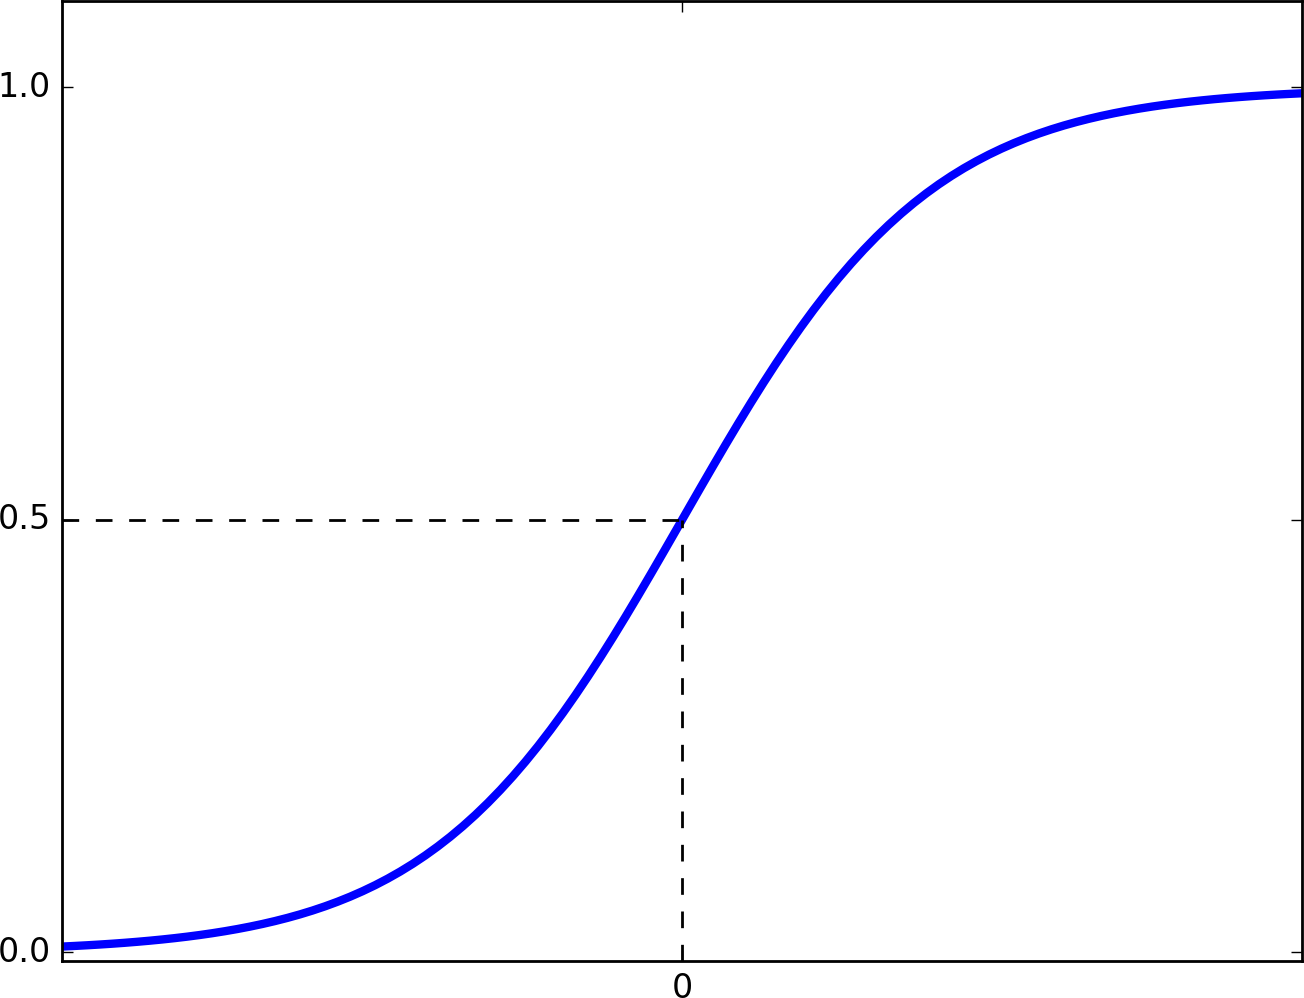
\includegraphics[height=.4\textheight]{./fig/fig_sigm.png}
\end{figure}
\note{Remark that $0<h_\theta(x)<1$}
\end{frame}

\begin{frame}
\frametitle{Probabilistic interpretation}
$$
h_\theta(x) =  \frac{1}{1 + \exp(-\theta^Tx)}
$$

\begin{block}{}
$h_\theta(x)$ can be interpereted as the probability that $y=1$ knowning $x$:

$$
h_\theta(x) = P(Y=1 | x ; \theta)
$$
\end{block}
Example:\\
If $ x = \left( \begin{array}{c}1 \\ \text{body temperature} \end{array} \right)$,
$h_\theta(x) = 0.6$ means that the probability to be sick given the temperature (and the paramter $\theta$) is 0.6.\\
\vspace{1em}
Note: Consequently, we have, $P(Y=0|x;\theta) = 1 - h_\theta(x)$
\end{frame}

\begin{frame}
\frametitle{Predicting the output $y$}
\begin{block}{}
In order to predict an ouptut $y \in \{0;1\}$, the following rule is used:
\begin{itemize}
\item if  $h_\theta(x) \geq 0.5$, we predict 1.
\item if  $ h_\theta(x) < 0.5$, we predict 0. 
\end{itemize}
\end{block}

Note: $h_\theta(x) \geq 0.5 \Leftrightarrow \theta^Tx \geq 0$

\note{make the demonstration of the note}

\end{frame}

\begin{frame}
\frametitle{Decision boundary}
\begin{columns}
\column{.5\textwidth}

\begin{figure}
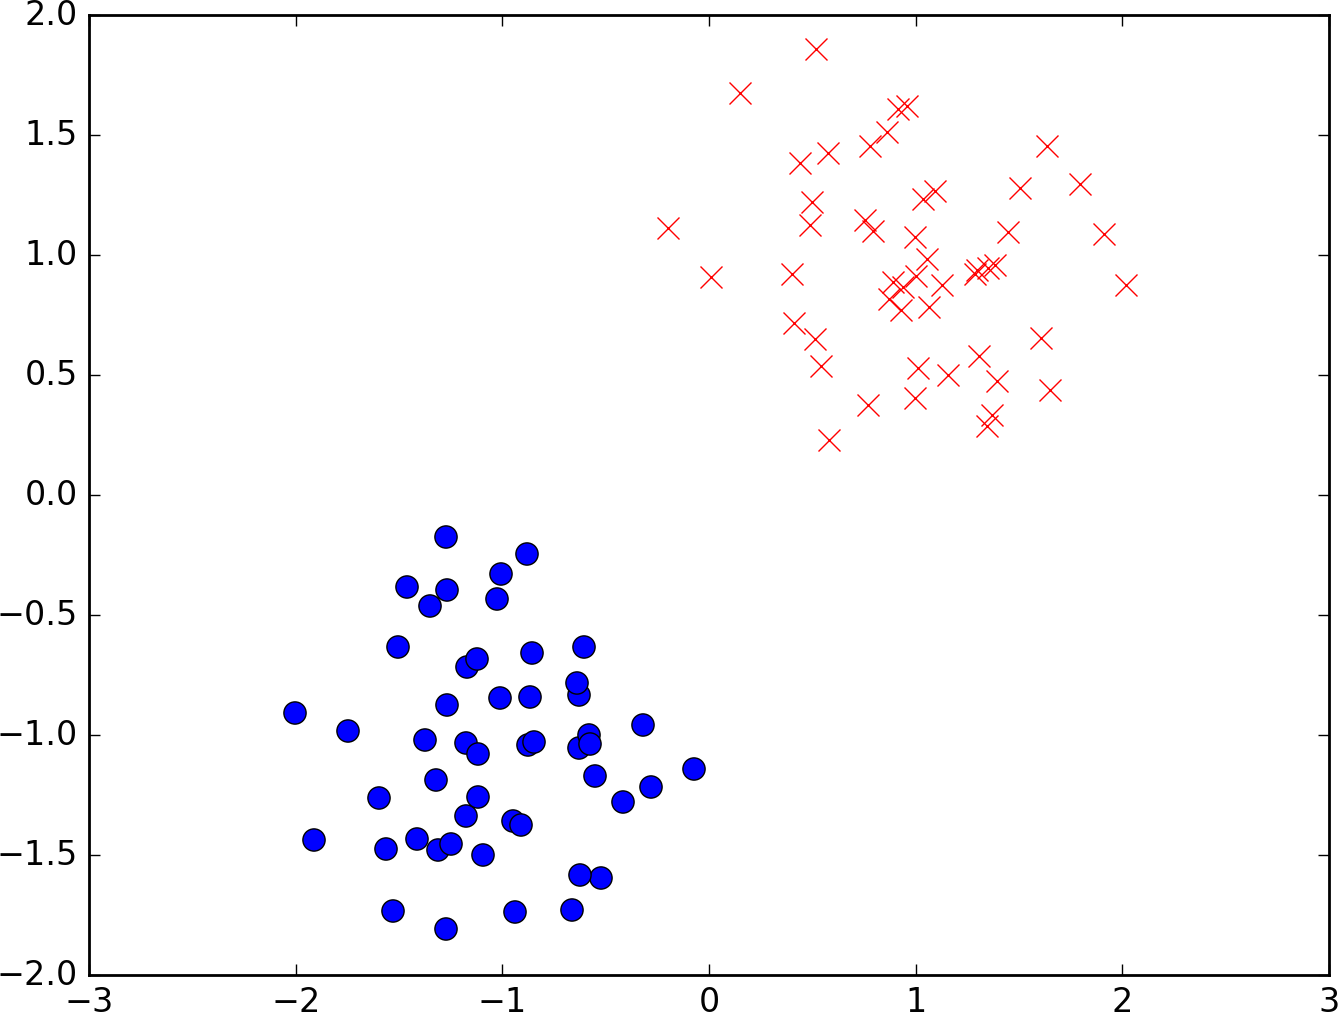
\includegraphics[width=.9\textwidth]{./fig/fig_2cl_nonoise.png}
\end{figure}

\column{.5\textwidth}
$$
h_\theta(x) = g(\theta_0 + \theta_1 x_1 + \theta_2 x_2)
$$
with $\bm{\theta} = (0,1,1)^T$
\end{columns}
The system predicts $y=1$ if $x_1 + x_2 \geq 0$
\begin{block}{}
The \alert{Decision boundary} is the line defined by the equation $x_1+x_2 =0$
\end{block}

\begin{alertblock}{}
Using logistic regression, the boundary is always linear (an hyperplane of the space)
\end{alertblock}

\end{frame}

\begin{frame}
\frametitle{Limits of the linear decision boundary }

\begin{columns}[t]
\column{.3\textwidth}
\begin{figure}
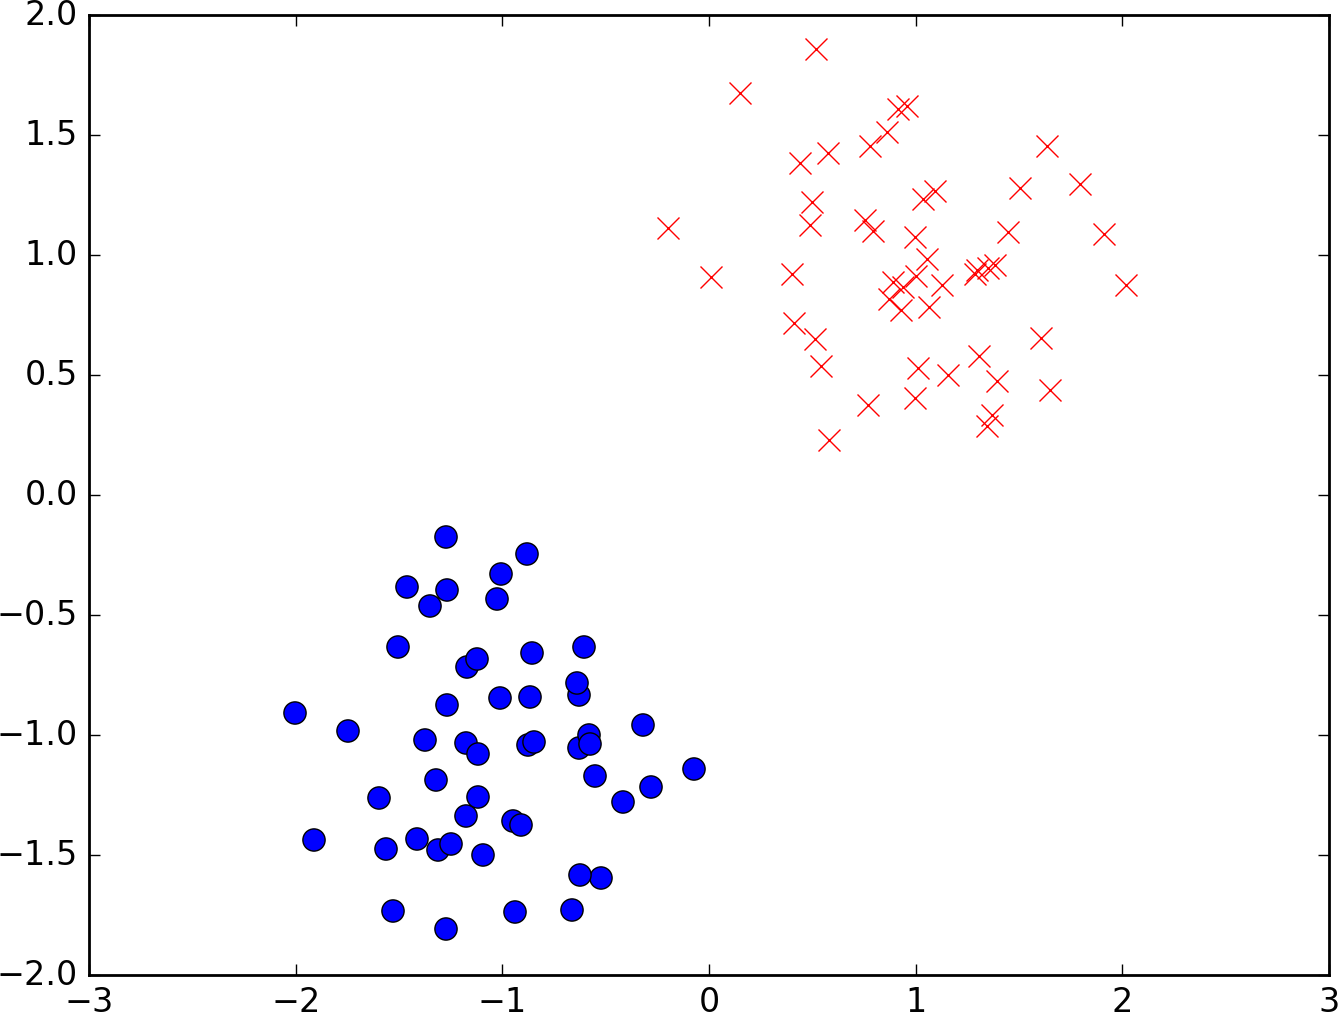
\includegraphics[width=.99\textwidth]{./fig/fig_2cl_nonoise.png}\\
Linear decision boundary  perfectly discrimates the two classes
\end{figure}
\column{.3\textwidth}
\begin{figure}
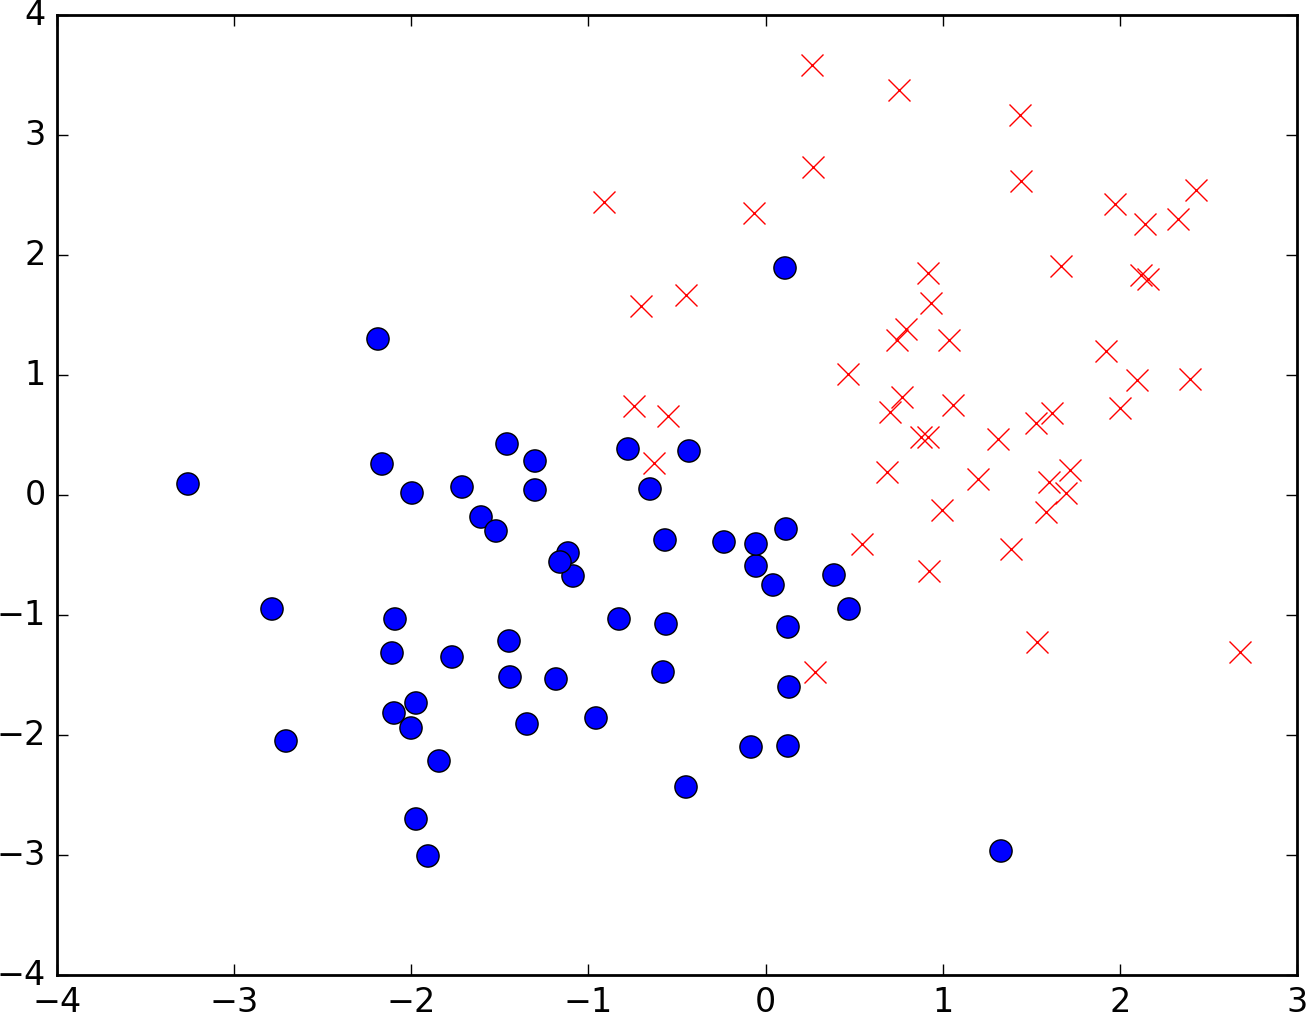
\includegraphics[width=.99\textwidth]{./fig/fig_2cl_noise.png}\\
Linear decision boundary is still relevant but some mis-classification can occur.
\end{figure}
\column{.3\textwidth}
\begin{figure}
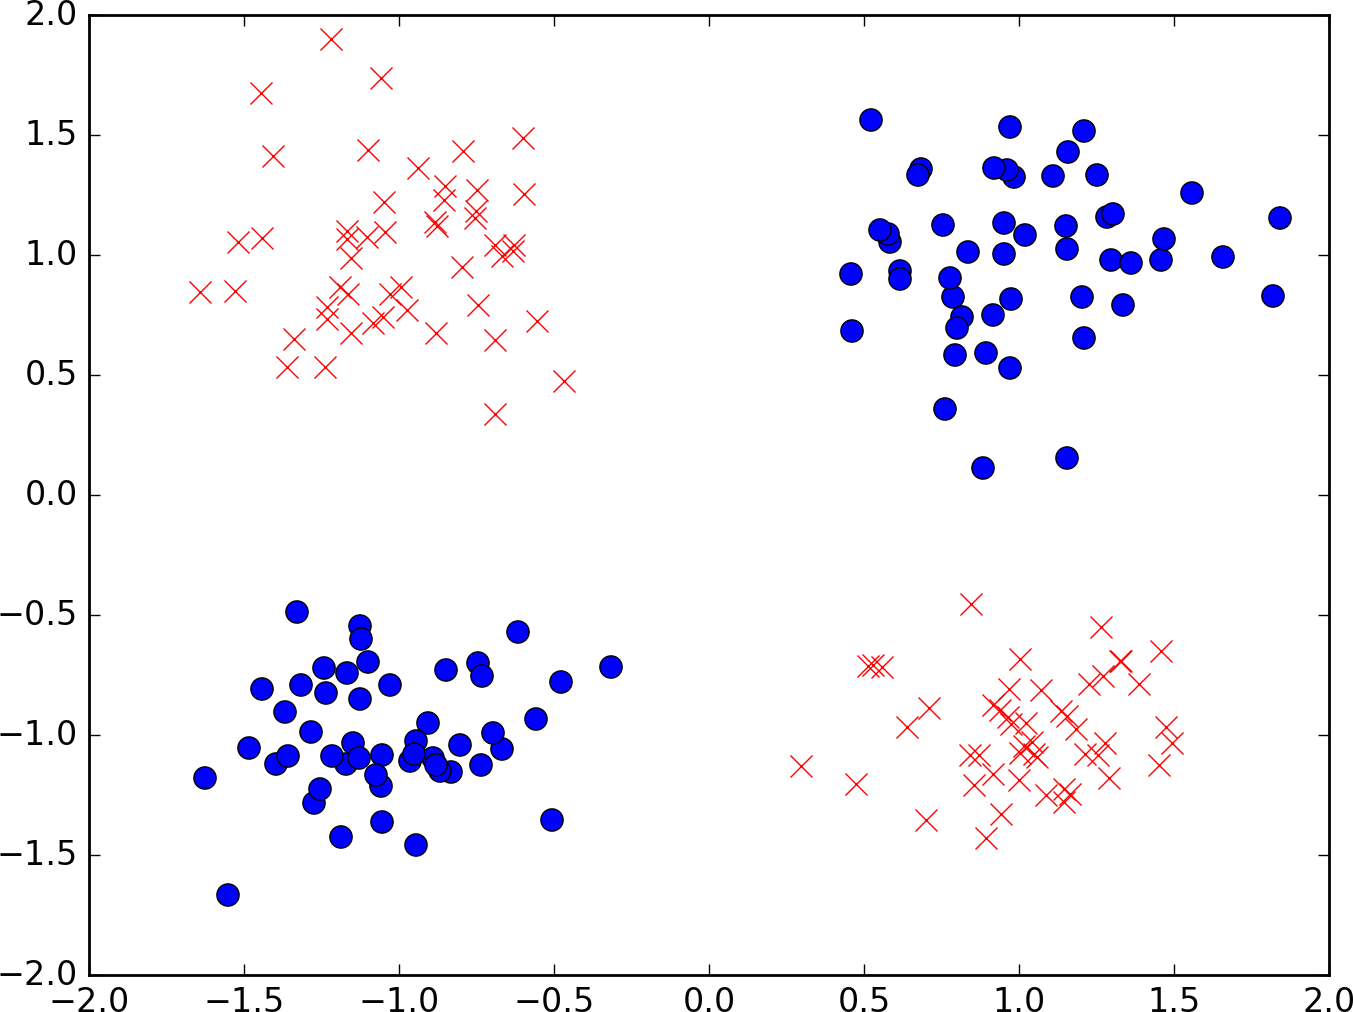
\includegraphics[width=.99\textwidth]{./fig/fig_4cl_nonoise.png}\\
Linear decision boundary is irrelevant, the logistic regression will fail.
\end{figure}
\end{columns}
\end{frame}

\begin{frame}
\frametitle{Choosing the parameters $\theta$}
\begin{itemize}
\item The training set $\{(x_1,y_1),\ldots,(x_n,y_n)\}$
\item The hypothesis representation: $\hat{y}=h_\theta(x) = g(\theta^Tx)$, $\theta \in \R^p$
\end{itemize}
\begin{block}{}
The determination of the "optimal" $\theta$ is made by minimizing a cost function:
$$
J(\theta) = \frac{1}{n} \sum_{i=1}^{n} D(h_\theta(x_i),y_i)
$$
where $D$ is a misfit function between the target output $y$ and the output of the classifier $h_\theta(x)$
\end{block}

Note, if we take the least-square cost function: $D(\hat{y},y)= \frac{1}{2}(\hat{y} - y)^2$, the cost function
is equivalent to the linear regression cost function.

\begin{exampleblock}{}
Is it relevant to take the least-square function?
\end{exampleblock}

\end{frame}

\begin{frame}
\frametitle{Problem with the least-square cost function}
\begin{itemize}
\item First problem (practical): the function is non-convex and the minimum is unclear
\begin{figure}
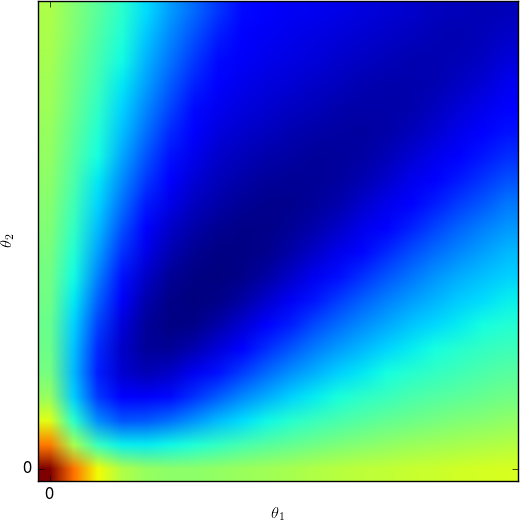
\includegraphics[height=.5\textheight]{./fig/cost_lmsq.png}
\end{figure}
\item Second problem (theorical): the mimimum of this cost function is not the maximum
likekihood estimator

\end{itemize}
\note{explain the example,draw other non-convex function, remind likelihood}
\end{frame}

\begin{frame}
\frametitle{Logistic regression cost function}
\framesubtitle{A intuitive definition}
For logistic regression, the cost function is contructed as follow:
\begin{itemize}
\item $D(h_\theta(x),y=1) = -\log(h_\theta(x))$
\item $D(h_\theta(x),y=0) = -\log(1-h_\theta(x))$
\end{itemize}
\begin{columns}
\column{.5\textwidth}
\begin{figure}
If $y=1$\\
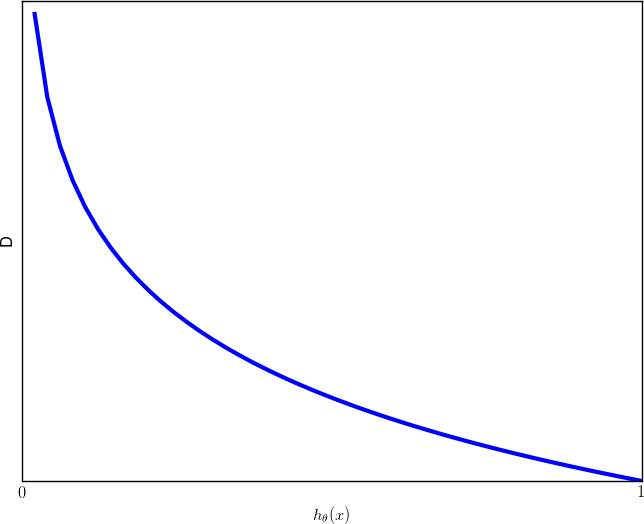
\includegraphics[height=.5\textheight]{./fig/cost1.png}
\end{figure}
\column{.5\textwidth}
\begin{figure}
If $y=0$\\
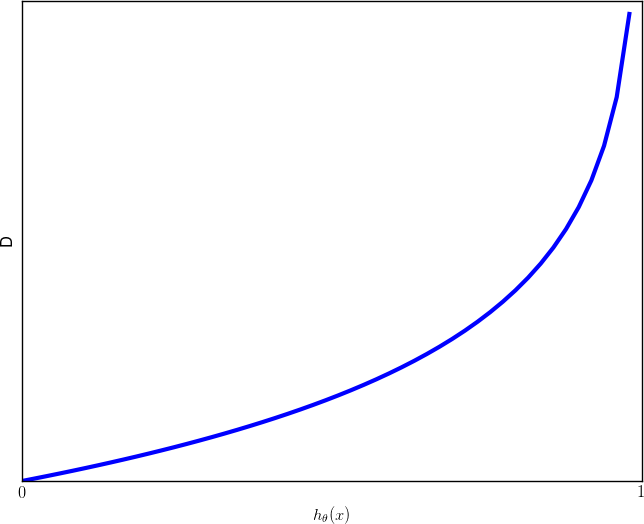
\includegraphics[height=.5\textheight]{./fig/cost0.png}
\end{figure}
\end{columns}
\note{Make comments on the different values and the limits}
\end{frame}

\begin{frame}
\frametitle{Logistic cost function}
 \framesubtitle{A compact definition}
The logistic cost function can be rewritten:
$$
D(h_\theta(x),y) = -y\log(h_\theta(x)) - (1-y)\log(1-h_\theta(x))
$$
\begin{itemize}
\item The value $\theta$ that minimize this cost function is the maximum of likelkihood
(maximum of $P(y|x,\theta$)
\item If we consider that $h_\theta(x)$ is a probability $q_1$ of the prediction $\hat{y}$ to be one.
We have a "true" probability $p_{y=1}=y$. Minimizing $D$ is equivalent to minimizing to cross-entropy
between $p$ and $q$.
\end{itemize}
\note{detail each point}
\end{frame}

\begin{frame}
\frametitle{The cost function}
\begin{columns}[t]
\column{.5\textwidth}
\begin{figure}
Points to classify:\\
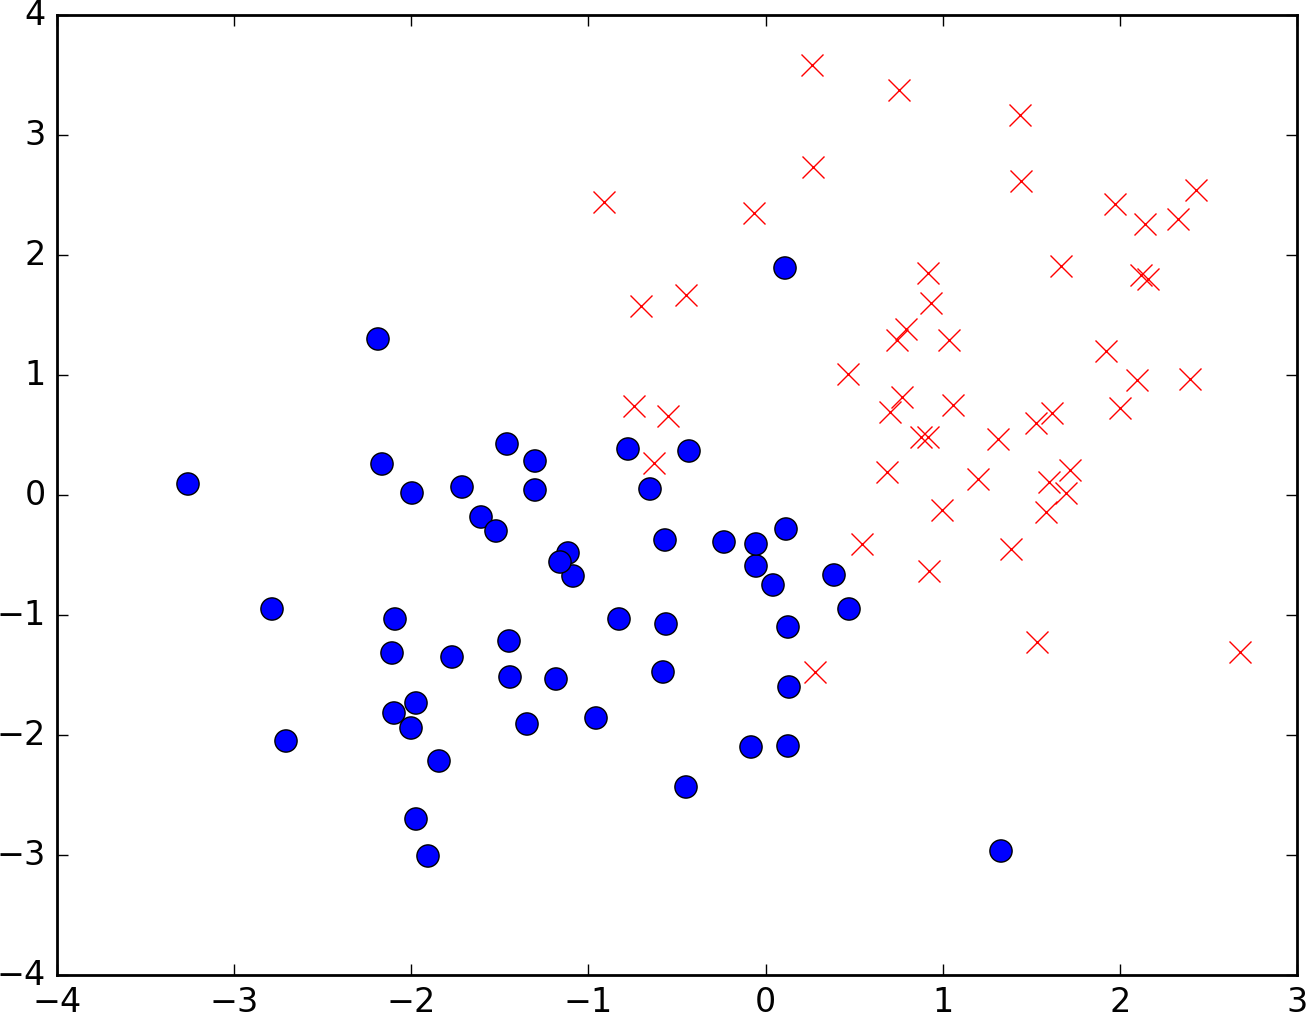
\includegraphics[width=.99\textwidth]{./fig/fig_2cl_noise.png}\\

model : $h_\theta(x)=\theta_1 x_1 + \theta_2 x_2$
\end{figure}

\column{.5\textwidth}
\begin{figure}
The cost unction to minimize:\\
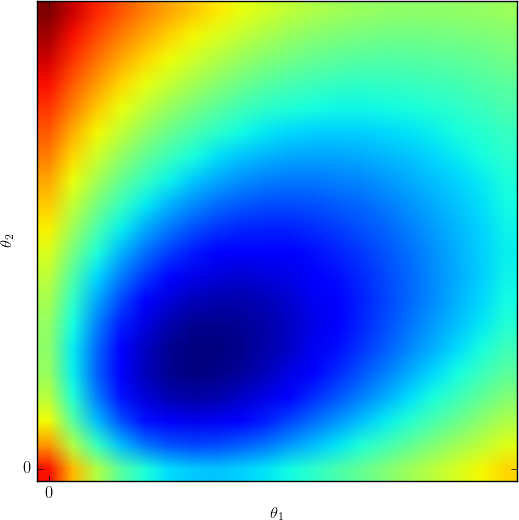
\includegraphics[width=.99\textwidth]{./fig/cost_log.png}\\

\end{figure}

\end{columns}

\end{frame}

\begin{frame}
\frametitle{Gradient descent}
\end{frame}

\begin{frame}
\frametitle{Gradient algorithm}
\end{frame}

\begin{frame}
\frametitle{Problems with the gradient algorithm}
\begin{itemize}
\item The method is sensitive to different order of magnitude for the different coordinates in
$x$.
\item There is an hyper-parameter to determine : the learning rate $\mu$
\item For large samples, the convergence is very long

\end{itemize}
\end{frame}

\begin{frame}
\frametitle{Scaling of $x$}
Two kind of scaling
reduce
minmax
\end{frame}

\begin{frame}
\frametitle{Scaling of $x$}
Two kind of scaling
reduce
minmax
\end{frame}

\begin{frame}
\frametitle{The learning rate $\mu$}
Other optimisation algorithmss (more complex)
\end{frame}

\begin{frame}
\frametitle{Computation cost}
Stochastic gradient
\end{frame}

\begin{frame}
\frametitle{Stochastic gradient algorithm}
\end{frame}

\end{document}